%%%%%%%%%%%%%%%%%%%%%%%%%%%%%%%%%%%%%%%%%%%%%%%%%%%%%%%%
%%%%%%%%%%%%%%%%%%%%%%%%%%%%%%%%%%%%%%%%%%%%%%%%%%%%%%%%
%%%%%%%%%%%%%%%%%%%%%%%%%%%%%%%%%%%%%%%%%%%%%%%%%%%%%%%%
\chapter{Hypothesis Testing}
\label{chap:hypo}

%%%%%%%%%%%%%%%%%%%%%%%%%%%%%%%%%%%%%%%%%%%%%%%%%%%%%%%%
%%%%%%%%%%%%%%%%%%%%%%%%%%%%%%%%%%%%%%%%%%%%%%%%%%%%%%%%
\section{\texorpdfstring{$Z$}{Z}-Test}
\label{hypo:Z_test}
% TODO

%%%%%%%%%%%%%%%%%%%%%%%%%%%%%%%%%%%%%%%%%%%%%%%%%%%%%%%%
%%%%%%%%%%%%%%%%%%%%%%%%%%%%%%%%%%%%%%%%%%%%%%%%%%%%%%%%
\section{Student's \texorpdfstring{$t$}{t}-Test}
\label{hypo:t_test}
Student's $t$-test can be used to
statistically compare the means of two samples via the $t$-distribution
given a $t$-statistic and degrees of freedom $\nu$.
The $t$-test is appropriate when each sample is small\footnote{For
larger sample sizes the $t$-distribution approaches the normal distribution which should be used instead.}, $n \lesssim 30$,
and drawn from a larger normally distributed population with an unknown standard deviation.
The \pvalue returned by the test estimates the probability of obtaining the sample means
assuming the null hypothesis, typically that the samples share the same mean, is true.
We can compute two-sided, \ie the means are not equal, or one-sided, \ie mean 1 is $>$ or $<$ mean 2,
forms of the $t$-test in three basic variations.
See \cref{fig:two_sided_t_test} for an illustration of a two-sided test's null hypothesis rejection regions.
The \texttt{scipy.stats.ttest\_*}
\href{https://docs.scipy.org/doc/scipy/reference/stats.html#statistical-tests}{family of functions}
to easily compute $t$-statistic and \pvalue in practice.

% TODO may want to switch to a similar figure in the Z-test section...
\begin{figure}
\centering
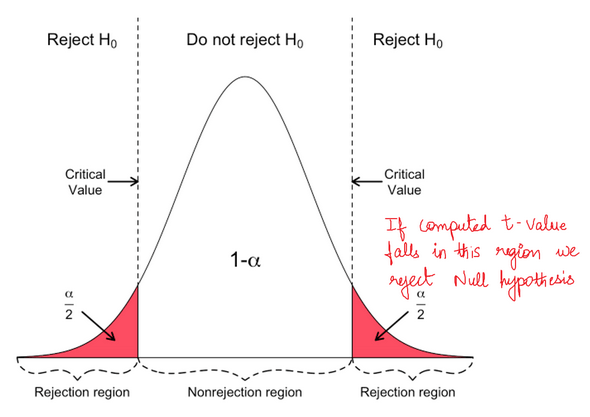
\includegraphics[width=0.7\textwidth]{figures/stats/one_side_t_test_rejection_regions.png}
\caption{
Illustration of a two-tail $t$-test's null hypothesis, $H_{0}$ rejection regions,
by \href{https://www.machinelearningplus.com/statistics/t-test-students-understanding-the-math-and-how-it-works/}{Selva Prabhakaran}.
In a one-tail $t$-test we would only consider the tail on a single side.
$\alpha$ is the significance level, typically \num{0.05} or lower.
}
\label{fig:two_sided_t_test}
\end{figure}

%%%%%%%%%%%%%%%%%%%%%%%%%%%%%%%%%%%%%%%%%%%%%%%%%%%%%%%%
\subsection{One-Sample}
\label{hypo:t_test:one}
In a one-sample $t$-test we have one sample of size $n$ with mean $\expval{x}$ and standard deviation $s$,
and test the null hypothesis that it belongs to a parent population with mean $\mu_{0}$.
In this case the parent population does not need to be normally distributed, but the distribution of possible $\expval{x}$ is assumed to be normal.

The $t$-statistic \cref{eq:hypo:t:one} can be used with $\nu = n-1$ to find a $\pvalue$.

\begin{equation}\label{eq:hypo:t:one}
t = \frac{\expval{x} - \mu_{0}}{s / \sqrt{n}}
\end{equation}

%%%%%%%%%%%%%%%%%%%%%%%%%%%%%%%%%%%%%%%%%%%%%%%%%%%%%%%%
\subsection{Two-Sample: Unpaired}
\label{hypo:t_test:two:unpaired}
In a two-sample unpaired $t$-test we have two independent samples, each of size $n$,
but with their own sample means $\expval{x_{i}}$ and standard deviations $s_{i}$.
Provided that we can assume that the two parent distributions of $x_{1}$ and $x_{2}$ have the same variance,
we can test the null hypothesis that the two parent distribution means are equal.

The $t$-statistic \cref{eq:hypo:t:two:unpaired} can be used with $\nu = 2n-2$ to find a $\pvalue$.

\begin{subequations}\label{eq:hypo:t:two:unpaired}
\begin{align}
t &= \frac{\expval{x_{1}} - \expval{x_{2}}}{s_{p} \sqrt{2/n}} \label{eq:hypo:t:two:unpaired:t} \\
s_{p} &= \sqrt{\left(s^{2}_{x_{1}} + s^{2}_{x_{2}}\right)/2} \label{eq:hypo:t:two:unpaired:s_p}
\end{align}
\end{subequations}

%%%%%%%%%%%%%%%%%%%%%%%%%%%%%%%%%%%%%%%%%%%%%%%%%%%%%%%%
\subsubsection{Different Sample Sizes}
\label{hypo:t_test:two:unpaired:diff_n}
If we relax the sample size condition and let $n_{1} \neq n_{2}$
we can still compute a $t$-statistic,
provided the parent distribution's variances are equal\footnote{A useful rule of thumb is $1/2 < s_{x_{1}} / s_{x_{2}} < 2$.}.

The $t$-statistic \cref{eq:hypo:t:two:unpaired:diff_n} can be used with $\nu = n_{1} + n_{2} - 2$ to find a $\pvalue$.

\begin{subequations}\label{eq:hypo:t:two:unpaired:diff_n}
\begin{align}
t &= \frac{\expval{x_{1}} - \expval{x_{2}}}{s_{p} \sqrt{\frac{1}{n_{1}} + \frac{1}{n_{2}}}} \label{eq:hypo:t:two:unpaired:diff_n:t} \\
s_{p} &= \sqrt{\left(\left(n_{1} - 1\right)s^{2}_{x_{1}} + \left(n_{2} - 1\right)s^{2}_{x_{2}}\right)/\left(n_{1} + n_{2} -2\right)} \label{eq:hypo:t:two:unpaired:diff_n:s_p}
\end{align}
\end{subequations}

%%%%%%%%%%%%%%%%%%%%%%%%%%%%%%%%%%%%%%%%%%%%%%%%%%%%%%%%
\subsubsection{Different Sample Sizes and Variances (Welch's \texorpdfstring{$t$}{t}-test)}
\label{hypo:t_test:two:unpaired:diff_n_diff_var}
If we further relax the assumptions and also let the population variances differ
we arrive at Welch's $t$-test which approximates\footnote{The
true distribution of $t$ depends somewhat on the unknown population variances,
see the \href{https://en.wikipedia.org/wiki/Behrens\%E2\%80\%93Fisher_problem}{Behrens--Fisher problem}
for more.} the $t$-distribution.

The $t$-statistic \cref{eq:hypo:t:two:unpaired:diff_n_diff_var:t} can be used with $\nu$ \cref{eq:hypo:t:two:unpaired:diff_n_diff_var:dof} to find a $\pvalue$.

\begin{subequations}\label{eq:hypo:t:two:unpaired:diff_n_diff_var}
\begin{align}
t &= \frac{\expval{x_{1}} - \expval{x_{2}}}{\sqrt{\frac{s^{2}_{1}}{n_{1}} + \frac{s^{2}_{2}}{n_{2}}}} \label{eq:hypo:t:two:unpaired:diff_n_diff_var:t} \\
\nu &= \frac{\left(s^{2}_{1}/n_{1} + s^{2}_{2}/n_{2}\right)^{2}}{\frac{\left(s^{2}_{1}/n_{1}\right)^{2}}{n_{1}-1} + \frac{\left(s^{2}_{2}/n_{2}\right)^{2}}{n_{2}-1}} \label{eq:hypo:t:two:unpaired:diff_n_diff_var:dof}
\end{align}
\end{subequations}

%%%%%%%%%%%%%%%%%%%%%%%%%%%%%%%%%%%%%%%%%%%%%%%%%%%%%%%%
\subsection{Two-Sample: Paired}
\label{hypo:t_test:two:paired}
In a two-sample paired $t$-test we have two dependent samples,
such as two sets of measurements from the same $n$ individuals taken at different times.
In this case, we are testing the null hypothesis that the difference in means of the two dependent samples is $\mu_{0}$.
Note, we can set $\mu_{0} = 0$ if we simply want to test for a statistically significant difference, and not an \apriori degree of difference.
Defining the difference between paired observations as $x_{\Delta}$, we compute the mean difference $\expval{x_{\Delta}}$ and $s_{\Delta}$ standard deviation on the sample.

The $t$-statistic \cref{eq:hypo:t:two:paired} can be used with $\nu = n-1$ to find a $\pvalue$.

\begin{equation}\label{eq:hypo:t:two:paired}
t = \frac{\expval{x_{\Delta}} - \mu_{0}}{s_{\Delta} / \sqrt{n}}
\end{equation}

%%%%%%%%%%%%%%%%%%%%%%%%%%%%%%%%%%%%%%%%%%%%%%%%%%%%%%%%
%%%%%%%%%%%%%%%%%%%%%%%%%%%%%%%%%%%%%%%%%%%%%%%%%%%%%%%%
\section{\texorpdfstring{$\chi^{2}$-Test}{Chi-Squared Test}}
\label{hypo:chi2_test}

Pearson's $\chi^{2}$-test can be used to
statistically compare a set of observations in
$n$ variables, $x_{i}$, to prior expectations via the $\chi^{2}$-distribution.
The \pvalue returned by the test estimates the probability of obtaining the observations
assuming the null hypothesis, \ie the expectations, is true.
The $\chi^{2}$-test statistic, $X^{2}$, is created with the assumption that
the data are normally distributed and independent,
which often is the case due to the central limit theorem.
It is constructed by squaring the difference\footnote{Yates's
correction for continuity $\left(x^{\text{obs}}_{j} - x^{\text{exp}}_{j}\right)^{2} \to \left(\abs{x^{\text{obs}}_{j} - x^{\text{exp}}_{j}}-0.5\right)^{2}$ may
also be applied in some low statistics cases.} between
an expected value, $x^{\text{exp}}_{i}$, and its corresponding observation, $x^{\text{obs}}_{i}$,
and dividing by the expectation:

\begin{equation}\label{eq:hypo:chi2_score}
X^{2} = \sum_{i=1}^{n} \frac{\left(x^{\text{obs}}_{i} - x^{\text{exp}}_{i}\right)^{2}}{x^{\text{exp}}_{i}}\,.
\end{equation}

In the limit that each $x^{\text{obs}}_{i}$ is normally distributed and $n$ is large, $X^{2} \to \chi^{2}$.
We can then use the $\chi^{2}$ distribution with $\nu = n-1$ degrees of freedom to find the \pvalue as the area to the right of $X^{2}$.
An easy way to compute $X^{2}$ and the \pvalue is to use the \texttt{scipy.stats.chisquare(f\_obs, f\_exp)}
\href{https://docs.scipy.org/doc/scipy/reference/generated/scipy.stats.chisquare.html}{function}.

The $\chi^{2}$-test can also be used to test of the data's independence, or homogeneity,
for $m$ samples of $n$ variables with $\nu = \left(n-1\right)\left(m-1\right)$ and\footnote{Note this is really the same as \cref{eq:hypo:chi2_score} if we reindex, just with a different $\nu$.}

\begin{equation}\label{eq:hypo:chi2_score_ind}
X^{2} = \sum_{i=1}^{n} \sum_{j=1}^{m} \frac{\left(x^{\text{obs}}_{i,j} - x^{\text{exp}}_{i,j}\right)^{2}}{x^{\text{exp}}_{i,j}}\,.
\end{equation}

%%%%%%%%%%%%%%%%%%%%%%%%%%%%%%%%%%%%%%%%%%%%%%%%%%%%%%%%
%%%%%%%%%%%%%%%%%%%%%%%%%%%%%%%%%%%%%%%%%%%%%%%%%%%%%%%%
\section{Binomial Proportion Test}
\label{hypo:binomial_test}
When dealing with samples of $n$ binary events we can perform hypothesis testing
on the number of observed positive events $k$
using test statistics built on the binomial distribution.

%%%%%%%%%%%%%%%%%%%%%%%%%%%%%%%%%%%%%%%%%%%%%%%%%%%%%%%%
\subsection{Exact Binomial Test}
\label{hypo:binomial_test:exact}
For small $n$ it is possible to compute the \pvalue
explicitly from the binomial distribution \cref{eq:stats:binomial}.
We test the null hypothesis that the probability of success is $\pi_{0}$
having actually observed $k$ successes, $k = n \pi$.

The \pvalue is then the sum

\begin{equation}\label{eq:hypo:binomial_test:exact}
\pvalue = \sum_{i \in \, \mathcal{I}} {n \choose i}\pi_{0}^{i} \left(1-\pi_{0}\right)^{n-i},
\end{equation}

\noindent where $\mathcal{I}$ depends on the type of test:

\begin{table}[H]
\centering
\begin{tabular}{l|l}
$\pi < \pi_{0}$ & $\mathcal{I} = \left\{0, 1, \ldots, k\right\}$, \\
$\pi > \pi_{0}$ & $\mathcal{I} = \left\{k, k+1, \ldots, n\right\}$, \\
$\pi \neq \pi_{0}$ & $\mathcal{I} = \left\{\forall \, i: P\left(x=i\right) \leq P\left(x = k\right)\right\}$, with binomial $P\left(x\right)$ \cref{eq:stats:binomial}.
\end{tabular}
\end{table}

%%%%%%%%%%%%%%%%%%%%%%%%%%%%%%%%%%%%%%%%%%%%%%%%%%%%%%%%
\subsection{One-Sample}
\label{hypo:binomial_test:one}
For large sample sizes the binomial distribution is approximated by the normal distribution
and we can use a form of the $Z$-test to produce {\pvalue}s.
We require the observations to be independent,
\ie we may only sample $< \SI{10}{\percent}$ of the parent population,
the sampling distribution of $\pi$ to be approximately normal,
and that there are $\geq 10$ successes and $\geq 10$ failures,
$n \pi_{0} \geq 10$ and $n \left(1-\pi_{0}\right) \geq 10$, \ie the success-failure condition.

The $Z$-score is then:

\begin{equation}\label{eq:hypo:binomial_test:one}
Z = \frac{\pi - \pi_{0}}{\sqrt{\pi_{0}\left(1-\pi_{0}\right)/n}} = \frac{k - n \pi_{0}}{\sqrt{n\pi_{0}\left(1-\pi_{0}\right)}}.
\end{equation}

Note that the one-sample test is provided by the
\texttt{scipy.stats.binomtest} \href{https://docs.scipy.org/doc/scipy/reference/generated/scipy.stats.binomtest.html}{function}.

%%%%%%%%%%%%%%%%%%%%%%%%%%%%%%%%%%%%%%%%%%%%%%%%%%%%%%%%
\subsection{Two-Sample}
\label{hypo:binomial_test:two}
In the case of two samples, we can test the null hypothesis
that the difference\footnote{Again, we set $\pi_{\Delta} = 0$ if we want to test for any difference.} in the sample's probabilities is $\pi_{\Delta}$.
We require that the $\pi$ from the two samples are uncorrelated,
have approximately normal sampling distributions,
and that their difference $\pi_{1} - \pi_{2}$ is an unbiased estimator.

The $Z$-score is then:

\begin{subequations}\label{eq:hypo:binomial_test:two}
\begin{align}
Z &= \frac{\pi_{1} - \pi_{2} - \pi_{\Delta}}{\pi_{p} \left(1-\pi_{p}\right)\left(1/n_{1} + 1/n_{2}\right)} \label{eq:hypo:binomial_test:two:Z} \\
\pi_{p} &= \frac{k_{1} + k_{2}}{n_{1} + n_{2}} \label{eq:hypo:binomial_test:two:pi_p}
\end{align}
\end{subequations}

%%%%%%%%%%%%%%%%%%%%%%%%%%%%%%%%%%%%%%%%%%%%%%%%%%%%%%%%
%%%%%%%%%%%%%%%%%%%%%%%%%%%%%%%%%%%%%%%%%%%%%%%%%%%%%%%%
\section{Mann-Whitney U Test}
\label{hypo:mann_whitney_U_test}
% TODO

%%%%%%%%%%%%%%%%%%%%%%%%%%%%%%%%%%%%%%%%%%%%%%%%%%%%%%%%
%%%%%%%%%%%%%%%%%%%%%%%%%%%%%%%%%%%%%%%%%%%%%%%%%%%%%%%%
\section{Kolmogorov-Smirnov Test}
\label{hypo:KS_test}
% TODO

%%%%%%%%%%%%%%%%%%%%%%%%%%%%%%%%%%%%%%%%%%%%%%%%%%%%%%%%
%%%%%%%%%%%%%%%%%%%%%%%%%%%%%%%%%%%%%%%%%%%%%%%%%%%%%%%%
\section{Hypothesis Test Power Analysis}
\label{hypo:power}

In hypothesis testing, like binary classification, we can suffer from two types of errors;
Type I or false positives, and Type II or false negatives.
The probabilities of these errors are functions of the experimental design
and are important to understand before undertaking a study.
We label $\alpha$ as the probability of rejecting a true null hypothesis, \ie a type I error,
and $\beta$ as the probability of failing to reject a false null hypothesis, \ie a type II error.
See \cref{table:CM} for a graphical representation in the context of binary classification.

$\alpha$ is the easier parameter to understand and improve,
as it is just the \pvalue threshold we select before the study.
It is typical to use $\alpha \leq \num{0.05}$.
$\beta$ depends on many factors including
$\alpha$,
the magnitude of the underlying effect,
the measurement variance,
the model being utilized,
and the sample size $n$.
Instead of using $\beta$ directly we often talk about the statistical power of a hypothesis test, $1-\beta$,
\ie the probability of correctly rejecting a false null hypothesis.
$\num{0.8} < 1-\beta$ is a commonly used target for the power.
As experimenters, we can
try to improve our methods to reduce the measurement variance,
select a more appropriate model\footnote{Parametric
models tend to have higher powers than the equivalent non-parametric model.
% https://youtu.be/diRX_NesFkA?t=558
In particular, comparing
the Mann-Whitney U and unpaired $t$-test gives $\frac{\left(1-\beta\right)_{\text{MWU}}}{\left(1-\beta\right)_{t}} = \frac{3}{\pi} = \num{0.955}$,
%while comparing the Wilcoxon signed-rank and paired $t$-test gives $\frac{\left(1-\beta\right)_{\text{WSR}}}{\left(1-\beta\right)_{t}} = \frac{2}{\pi} = \num{0.6437}$, % TODo add if I cover the Wilcoxon signed-rank test in the future
for large $n$.},
or begrudgingly accept some combination of a larger $\alpha$ or larger minimal detectable difference.
However, the primary lever for improving an experiment's power is by increasing $n$,
at the cost of additional time and money to complete the study.

Calculating $\beta$ can be challenging and is commonly done in software\footnote{The \texttt{statsmodels.stats.power}
\href{https://www.statsmodels.org/dev/stats.html?highlight=statsmodels\%20stats\%20power\#power-and-sample-size-calculations}{module}
provides many useful functions, see \href{https://machinelearningmastery.com/statistical-power-and-power-analysis-in-python/}{here} for one example.} particular to the model being utilized.
For a simple example, we can consider a $Z$-test of a null hypothesis $\mu_{0}$
and compute the power of the test at a specific value of the alternative hypothesis $\mu_{a}$, with $\mu_{0} < \mu_{a}$.
For the given $\alpha$ being used we can look up the corresponding critical $Z$-score, $Z_{\alpha}$.
Then assuming a standard deviation of $s_{\text{est}}$ from prior work,
and knowing $n$, we can estimate the sample mean
which would put us at the critical $Z$-score, $\expval{x_{c}}$ \cref{eq:hypo:power_ex:x_c}.
We then calculate the $Z$-score again, this time assuming the alternative hypothesis $\mu_{a}$ is true
and we have observed $\expval{x_{c}}$ from our sample, \ie we are right at the edge of rejecting a false null hypothesis.
This $Z$-score, $Z_{a}$ \cref{eq:hypo:power_ex:Z_a}, can finally be used to find the power $1-\beta = P\left(Z_{a} < Z\right)$.

\begin{subequations}\label{eq:hypo:power_ex}
\begin{align}
Z_{\alpha} &= \frac{\expval{x_{c}} - \mu_{0}}{s_{\text{est}} / \sqrt{n}} \implies
\expval{x_{c}} = \frac{Z_{\alpha} s_{\text{est}}}{\sqrt{n}} + \mu_{0} \label{eq:hypo:power_ex:x_c} \\
Z_{a} &= \frac{\expval{x_{c}} - \mu_{a}}{s_{\text{est}} / \sqrt{n}}
= Z_{\alpha} + \sqrt{n}\,\frac{\mu_{0} - \mu_{a}}{s_{\text{est}}} \label{eq:hypo:power_ex:Z_a}
\end{align}
\end{subequations}

Note that as advertised $Z_{a}$ depends on
the choice of $\alpha$ via $Z_{\alpha}$,
the magnitude of the underlying effect $\mu_{0} - \mu_{a}$,
the measurement variance $s_{\text{est}}$,
the sample size $n$,
and is particular to this hypothesis test.
Plugging in numbers, if
$\alpha = \num{0.05} \to Z_{\alpha} = \num{1.645}$,
$\mu_{0} = \num{10}$,
$s_{\text{est}} \approx \num{2}$,
$n = \num{100}$,
and we want to find the power of the test for an alternative hypothesis of $\mu_{a} = \num{10.5}$,
we have $Z_{a} = \num{-0.8551} \to P\left(\num{-0.8551} < Z\right) = \num{0.8038}$
and thus the power is an acceptable $1-\beta = \num{0.8038} = \SI{80.38}{\percent}$.
We could use a similar line of reasoning to estimate
the $n$ necessary to obtain a desired $\alpha$ and $\beta$ before running the experiment.

% import numpy as np
% import scipy.stats
% norm = scipy.stats.norm
% Z_a = norm.ppf(1-0.05) + np.sqrt(100)*(10-10.5)/2
% print(f'Z_a = {Z_a:.4f}')
% print(f'Power = 1-beta = {1-norm.cdf(Z_a):.4f}')
